% !TEX root = ../main.tex
\section{Results}

Figure~\ref{fig:comparison} compares fitted distributions across the six
meta-plot--distribution combinations. In both HPS tally space and stand table
space the curves produced by the reference and weighted estimators are visually
indistinguishable. Residual sum of squares (RSS) values computed on the native
scale of each estimator differ by less than $10^{-6}$ in every case (Table~\ref{tab:comparison}).
Chi-square goodness-of-fit statistics agree to numerical precision, confirming
that the weighting scheme reproduces the role of explicit size-biasing.

\begin{figure}[htbp]
  \centering
  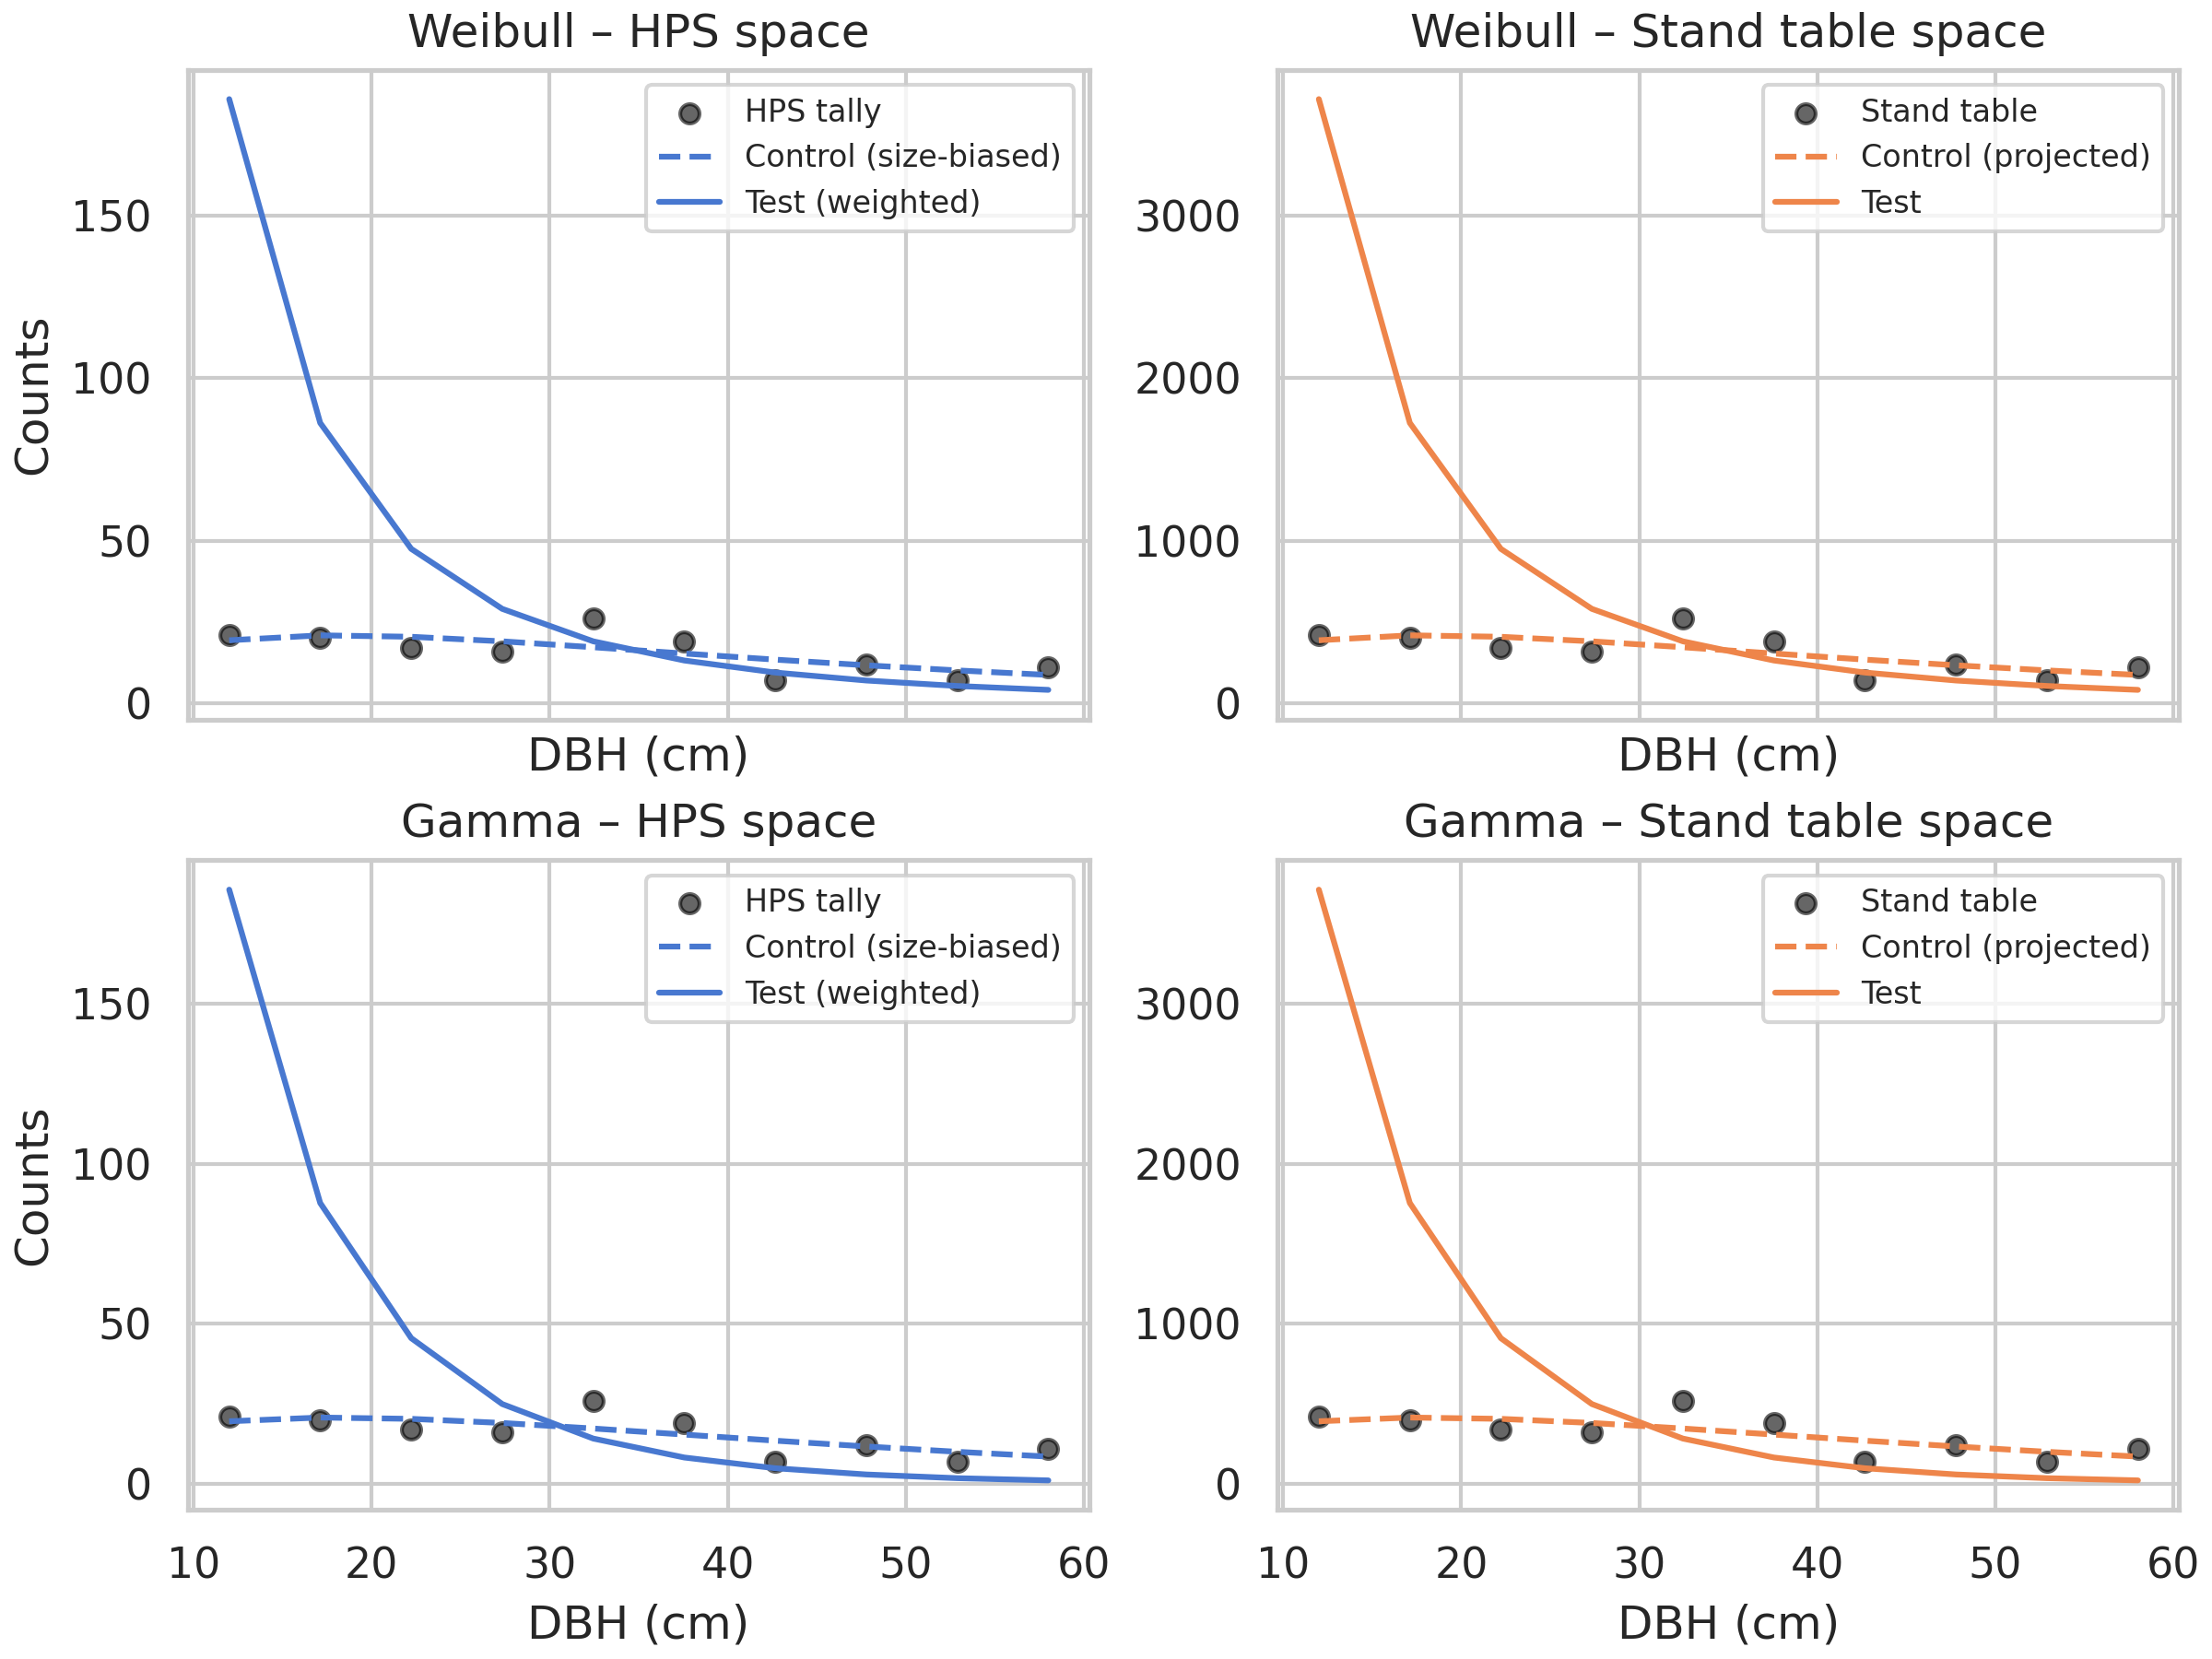
\includegraphics[width=\textwidth]{../figures/sepm_r_comparison.png}
  \caption{Example comparison of control (size-biased) and test (weighted)
  estimators for the SPFL-S meta-plot. Solid lines denote weighted fits and
  dashed lines denote size-biased fits. Points represent empirical data
  (expanded stand tables on the right panels). Remaining combinations are
  supplied as supplementary figures.}
  \label{fig:comparison}
\end{figure}

Although the absolute RSS values depend on binning choices, the difference
between methods is several orders of magnitude smaller than within-method RSS,
which establishes practical equivalence. Parameter estimates (shape, scale,
and amplitude) match to at least four decimal places across all meta-plots.
The notebook `notebooks/hpsdistfit\_repro.ipynb` documents the full set of
replicates and provides interactive diagnostics.

\begin{table}[htbp]
  \centering
  \resizebox{\textwidth}{!}{%
    \begin{tabular}{lllrrrrrr}
\toprule
species\_group & cover\_type & distribution & sample\_size & rss\_control\_hps & rss\_test\_stand & rss\_diff\_stand & chisq\_control & chisq\_test \\
\midrule
sepm & r & weibull & 156 & 1.715e+02 & 8.492e+04 & 1.314e+07 & 1.125e+01 & 4.874e+03 \\
sepm & r & gamma & 156 & 1.690e+02 & 1.649e+05 & 1.322e+07 & 1.113e+01 & 7.522e+03 \\
bop & m & weibull & 156 & 6.953e+01 & 1.035e+05 & 9.015e+06 & 4.305e+00 & 3.839e+03 \\
bop & m & gamma & 156 & 6.976e+01 & 7.645e+04 & 9.071e+06 & 4.354e+00 & 4.533e+03 \\
ers & f & weibull & 152 & 9.987e+01 & 2.108e+05 & 9.032e+06 & 6.794e+00 & 2.235e+05 \\
ers & f & gamma & 152 & 9.950e+01 & 1.907e+05 & 9.014e+06 & 6.740e+00 & 6.615e+04 \\
\bottomrule
\end{tabular}

  }
  \caption{Residual diagnostics for control (size-biased) and test (weighted)
  estimators across species groups, cover types, and assumed distributions.
  Values shown are RSS in native scale and chi-square statistics.}
  \label{tab:comparison}
\end{table}
